\chapter{Introduction} \label{chapter:introduction}

This chapter presents the motivation behind this
project~\ref{section:motivation}, the main
contributions~\ref{section:contribution} we hope to make with this work and a
brief outline~\ref{section:outline} on this document's structure.

\section{Motivation} \label{section:motivation}

The Hash Code programming competition is an yearly event held by Google where
teams are asked to solve complex and challenging engineering problems using any
tools and programming languages of their choice in four hours available.  The
problems are typically inspired by issues arising in real-world situations, such
as vehicle routing, task scheduling, and Wi-Fi router placement. They are posed
as ``open'' research problems for which there exists a variety of solutions of
different qualities. In fact, the great majority of these are essentially
Combinatorial Optimization (CO) problems concerning the search for the best
solutions among a potentially large set of candidate solutions, thus being of
utmost importance the adoption of efficient search strategies that take the
available time budget into account. Moreover, in the context of the competition,
the contestants must also read, understand the problem and find a suitable
representation for it, which is to say that, not all the available time will be
spent in the solution optimization stage.

For solving CO problems, a variety of algorithms exist that often offer a
compromise between the time and quality of the solutions found. The heuristics
are a set of procedures, often problem-specific, that attempt to quickly solve a
problem and provide a helpful ``rule of thumb'' for achieving decent results,
generally in a greedy fashion. A superset of these algorithms is called
meta-heuristics, and contrary to regular heuristics, these are generic and can
be applied to a broad range of problems. Natural processes and phenomena, such
as collective behavior, natural selection, and some physical properties of
materials, inspire several meta-heuristics search processes making them flexible
and adaptable, although more computationally intensive than heuristics.

A suite of optimization tools of different natures is available to practitioners
for solving CO problems, thus constituting a challenge to enumerate them all. In
particular, there exist a set of tools that rely upon more mathematical and
exact approaches yielding optimal solutions although not being used in a
competition context due to their poor time performance on challenging problems,
such as the Hash Code challenges.

In the context of the Google Hash Code competition, competitors frequently make
use of greedy and heuristic strategies tailored to the challenge.  Moreover,
meta-heuristics in this situation are not as popular due to the time constraints
imposed by the competition format. At first instance, the majority of
optimization problems are structurally different from each other, which makes it
demanding to write general-purpose heuristic solvers that can be easily reused.
On the other hand, it might not be worth the effort spent in the implementation
of such solvers and provided that the benefit of using a simple heuristic
strategy might outweigh the development and the running cost of meta-heuristic
solvers e.g., evolutionary algorithms.

Algorithms such as meta-heuristics usually follow some notion of an optimization
strategy that guides the procedure in the search for solutions.  Some of the
main strategies are constructive and local search.  Constructive search
algorithms work by starting with an empty or partially complete solution and
building a complete and feasible solution by iteratively adding components based
on the solution's current state and the problem's constraints.  In contrast,
local search algorithms develop a given initial solution to the problem by
introducing small changes that aim to improve it to a local optimum rather than
a global one.  A common usage of these strategies in competition is to sequence
them, starting with a constructive search stage, improving solutions to a
certain stagnation point and then taking advantage of a local search strategy in
an attempt to enhance the solutions even further.

\begin{figure}[h]
      \centering
      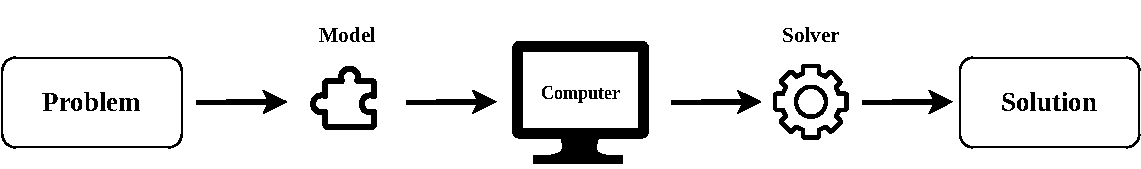
\includegraphics[width=\textwidth,keepaspectratio]{../assets/modelling/modelling.pdf}
      \caption{Modelling and Problem Solving}
      \label{fig:problem-solving}
\end{figure}

It is evident that algorithms or solvers that utilize these search strategies
are highly dependent on the specific problem they are trying to solve.  The
solver plays a crucial role in the problem-solving process as it is responsible
for finding a solution. However, without a comprehensive model that can provide
the solver with relevant information about the problem, the solver's
effectiveness may be impaired.

The model serves as a means of presenting the various aspects of the problem to
the computer, which will subsequently utilize a solver to find a
solution (~\ref{fig:problem-solving}).  When constructing a model, it is important
to include relevant features such as the representation of the problem and
solution, a description of how components can be added or removed from the
solution, and methods for evaluating the solution, calculating bounds, and
obtaining other heuristic information.

A good model should encode in it all the relevant information from the problem
and ask the right questions to obtain it, adhering to the philosophy that ---
``\textit{understanding the question is half the answer}''. Additionally, if a
model was to be built in a standardized way, this would allow the development of
a suite of generic and reusable (meta-heuristic) solvers that could find
solutions in a black-box fashion. This idea has already been explored to some
extent in previous work~\cite{outeiro2021application,vieira2009uma} and will be
further deepened.

It is worth noting that the modelling aspect in this field has often been
neglected by the community, which has been primarily focused on the development
of meta-heuristics algorithms (solvers). This discrepancy can be contrasted with
the mathematical perspective, where practitioners and researchers have
emphasized the importance of clearly separating the model and the algorithm
(solver), and have placed a significant emphasis on the modelling perspective.
This gap highlights the importance of considering the modelling aspect in this
field.

There has also been a recent growing interest within the community in the
development of optimization benchmark problems that are both relevant in
practical applications and amenable to theoretical analysis. The Hash Code
problems may be suitable candidates for this purpose, as they pose significant
challenges from a modelling perspective while also being easily describable.
Furthermore, these problems have already been partially solved in a competitive
setting and have a wealth of empirical data available on the most effective
known solutions.  Overall, these factors make the Hash Code problems an ideal
testing ground for both modelling and the evaluation of meta-heuristics.

\section{Contribution}
\label{section:contribution}

The main goal of this work is to develop and implement effective heuristic and
meta-heuristic approaches for solving Hash Code problems, with a particular
focus on the modelling aspect and the clear separation between solvers and
models.  By doing so, we hope to develop more structured and efficient
problem-solving strategies that can effectively address a range of challenges.
Additionally, some effort will be made to address other key areas that are
crucial to the success of this work, namely:

\begin{itemize}
      \item Development and refinement of the frameworks that separate models from solvers
            currently materialized in an Application Programming Interface (API)
            designed only for constructive search~\cite{outeiro2021application}.
            The main goal is to optimize and ``fine-tune'' this API in order to improve its
            efficacy and utility, by using the Hash Code problems as benchmarks.

      \item Expansion of the aforementioned API to support local search strategies
            in a problem-independent manner. This will allow for its application to a wider
            range of problems and contexts.

      \item Implementation of a small set of general-purpose meta-heuristic solvers and utilities
            that can be used to not only generate and test solutions for the multiple
            Hash Code benchmark problems, but also to verify the correctness of the results.
\end{itemize}

Last but not least, the objective of this work is to engage in a critical
examination of the strengths and limitations of our proposed approach to problem
modelling and solver development. This discussion will be relevant to
meta-heuristic researchers, software developers, and practitioners alike. The
analysis will consider various performance dimensions, including the effort
required for problem modelling and solver development, the computational
efficiency of the implemented software, and the quality of the solutions
obtained.

\section{Outline}
\label{section:outline}

The remainder of this document is structured as follows:

\begin{itemize}
      \item \textbf{Chapter~\ref{chapter:background}:} Provides some background
            on some essential aspects of optimization, search strategies,
            meta-heuristics, and modelling. Moreover, it presents the modelling
            frameworks and current state of the art of the API~\cite{outeiro2021application}~that
            supports this work.

      \item \textbf{Chapter~\ref{chapter:approach-objectives}:} Analyzes the main objectives
            that we hope to achieve, along with the methodology required to successfully
            accomplish them. In addition, a work plan is presented outlining the tasks to
            be carried out in the upcoming semester. Finally, some comments are made
            regarding the usability and ease of use of the tools that will be utilized,
            given their current state.

            % \item \textbf{Chapter~\ref{chapter:hashcode}:} Gives some insight
            %       into the Google Hash Code competition and typical problems presented to
            %       contestants. Furthermore, it makes a brief categorization of all the problems
            %       from previous editions, with particular emphasis on the ones analyzed so far.

      \item \textbf{Chapter~\ref{chapter:preliminary-work}:}
            Gives some insight into the Google Hash Code competition and typical
            problems presented to contestants. Furthermore, it makes a brief
            categorization of all the problems from previous editions, with particular
            emphasis on the ones analyzed so far. Finally, it describes the modelling
            of the problems examined and the results obtained

            % \item \textbf{Chapter~\ref{chapter:conclusion}:} Presents a summary of the work
            %       completed and some observations about the next steps to be taken.

      \item \textbf{Chapter~\ref{chapter:conclusion}:} Presents a brief reflection on this work.

\end{itemize}

